% Standalone TikZ figure: Overlap Concept (Venn diagram)
% Compile with: pdflatex overlap_concept_tikz.tex
\documentclass[tikz,border=5pt]{standalone}
\usepackage{tikz}
\usetikzlibrary{patterns, calc, positioning, decorations.pathreplacing}
\usepackage{amsmath,amssymb}

\begin{document}
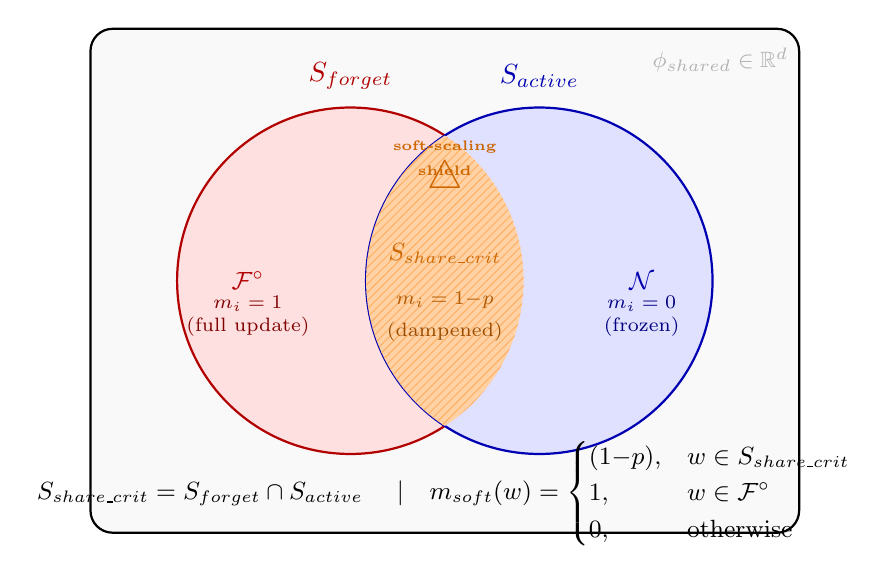
\begin{tikzpicture}[
    every node/.style={font=\small},
]

% === Main parameter space (large rectangle) ===
\draw[thick, rounded corners=8pt, fill=gray!5] (-4.5,-3.2) rectangle (4.5,3.2);
\node[font=\footnotesize\itshape, text=gray!60] at (3.5,2.8) {$\phi_{shared} \in \mathbb{R}^d$};

% === S_forget circle (left, red/orange) ===
\begin{scope}
    \clip (-1.2,0) circle (2.2cm);
    \fill[red!12] (-1.2,0) circle (2.2cm);
\end{scope}
\draw[thick, red!70!black] (-1.2,0) circle (2.2cm);

% === S_active circle (right, blue) ===
\begin{scope}
    \clip (1.2,0) circle (2.2cm);
    \fill[blue!12] (1.2,0) circle (2.2cm);
\end{scope}
\draw[thick, blue!70!black] (1.2,0) circle (2.2cm);

% === Intersection: S_share_crit (re-fill with pattern) ===
\begin{scope}
    \clip (-1.2,0) circle (2.2cm);
    \fill[orange!35] (1.2,0) circle (2.2cm);
    % Add diagonal pattern for emphasis
    \fill[pattern=north east lines, pattern color=orange!60] (1.2,0) circle (2.2cm);
\end{scope}

% === Labels for regions ===
% Forget-only region
\node[text=red!70!black, font=\small\bfseries, align=center] at (-2.5,0) {$\mathcal{F}^{\circ}$};
\node[text=red!50!black, font=\scriptsize, align=center] at (-2.5,-0.45) {$m_i = 1$\\(full update)};

% Critical overlap region
\node[text=orange!80!black, font=\small\bfseries, align=center] at (0,0.35) {$S_{share\_crit}$};
\node[text=orange!70!black, font=\scriptsize, align=center] at (0,-0.25) {$m_i = 1{-}p$};
\node[text=orange!60!black, font=\scriptsize, align=center] at (0,-0.65) {(dampened)};

% Active-only region
\node[text=blue!70!black, font=\small\bfseries, align=center] at (2.5,0) {$\mathcal{N}$};
\node[text=blue!50!black, font=\scriptsize, align=center] at (2.5,-0.45) {$m_i = 0$\\(frozen)};

% === Circle labels ===
\node[text=red!70!black, font=\normalsize\bfseries] at (-1.2,2.6) {$S_{forget}$};
\node[text=blue!70!black, font=\normalsize\bfseries] at (1.2,2.6) {$S_{active}$};

% === Shield icon on intersection ===
\node[font=\Large, text=orange!80!black] at (0,1.3) {$\bigtriangleup$};
\node[font=\tiny\bfseries, text=orange!80!black] at (0,1.7) {soft-scaling};
\node[font=\tiny\bfseries, text=orange!80!black] at (0,1.4) {shield};

% === Bottom equation ===
\node[font=\small, text=black] at (0,-2.7) {%
$S_{share\_crit} = S_{forget} \cap S_{active}$
\quad\textbar\quad
$m_{soft}(w) = \begin{cases}
(1{-}p), & w \in S_{share\_crit} \\
1, & w \in \mathcal{F}^{\circ} \\
0, & \text{otherwise}
\end{cases}$};

\end{tikzpicture}
\end{document}
